\section{Anforderungsmanagement}

Das Anforderungsmanagement, ist eine Management Disziplin die das Software Engineering unterstützt. Es setzt sich damit auseinander eine optimale Lösung durch strukturierte und organisierte Planung und Definition der Anforderung zu erreichen.

Durch das Anforderungsmanagement soll vermieden werden, dass durch schlechte, unzureichende oder missverständliche Definitionen, eine Entwicklung am Ende nicht dem Entspricht, was der Auftraggeber haben wollte.

Das Anforderungsmanagement lässt sich in unterschiedliche Arbeitspakete unterteilen, hierzu lassen sich in der Literatur die unterschiedliche Ausprägungen und Anzahlen finden. Bei Marcus Grande\autocite[10]{100minAM} wird in vier Haupttätigkeiten unterteilt. Für die Diplomarbeit habe ich mir beispielhaft die Punkte ausgesucht, wie sie im Buch "Anforderungsmanagement in sieben Tagen"\autocite[30-31]{AMin.sieben.T} zu finden sind.  


\subsection{Arbeitspakete im Anforderungsmanagement}
\begin{itemize}
\item Anforderungsmanagement planen \\
		Das Anforderungsmanagement dient der Planung und so ist es auch nicht weiter
		verwunderlich, dass auch in der Vorbereitung eine Planung für das Anforderungsmanagement
		sinnvoll ist. Es stehen eine Vielzahl von Tools, welche das Anforderungsmanagement
		unterstützen, die Art und weise der Dokumentation sollte festgelegt werden und die
		Anforderungsattribute sollten festgelegt werden.

\item Ausgangspunkt finden \\
		\textit{Um das Ziel zu finden, sollte man wissen wo man los geht} \\
		Bevor man mit der Zielfindung beginnen kann, sollte man wissen, wie der aktuelle Stand 
		ist. Man kann das mit einem Orientierungsmarsch bei der Bundeswehr vergleichen, bei dem 
		Soldaten mit einem Kompass und einer Geländekarte ein Ziel erreichen müssen, wenn sie 
		nicht wissen wo sie los gehen, ist es unwahrscheinlich, dass sie das ausgegebene Ziel 
		erreichen. Wie schaut der zu bearbeitende Prozess aus und wer ist darin Akteur und/oder 
		Betroffener. Durch das ermitteln des IST-Zustand kann man seine Stakeholder ermitteln, 
		lernt den Prozess im aktuellen Zustand, seine Grenzen und die von außen einwirkenden 
		Elemente kennen. 

\item Anforderungen erheben\\
		Für die Erhebung von Anforderungen existieren verschiedene Methoden und Quellen. 
		
		\textbf{Quellen} für Anforderungen sind 
		\begin{itemize}
		\itemsep-8pt
		\item Stakeholder, die Aufgrund ihrer Mitarbeit am Prozess oder durch Auswirkungen und 
		Ergebnissen dieses, betroffen sind.
		\item Prozessmodelle, in denen der Ablauf des Prozesses dokumentiert ist
		\item Beobachtungen des Prozessalltags
		\item Prozessbeschreibungen oder Problemberichte
		\end{itemize}		
		\textbf{Methoden} zur Erhebung von Anforderungen sind
		\begin{itemize}
		\itemsep-8pt
		\item Interviews mit Stakeholdern oder Verantwortlichen
		\item Workshops mit Stakeholdern 
		\item Analysen von Berichten und Beschreibungen
		\end{itemize}
		
		Je nach zur Verfügung stehender Quelle ist eine dazu passende Methode zur Erhebung 
		dieser anzuwenden.
		
\item Anforderungen dokumentieren\\
		Mit dem Erheben von Anforderungen wird auch das dokumentieren dieser zu einem Thema. 
		Wenn die Disziplin des Anforderungsmanagement in einem größeren Unternehmen schon weit
		fortgeschritten ist wird es für die Dokumentation evtl. schon geeignete Tools im 
		Unternehmen geben. Bei kleinen Firmen wird dies in der Regel wohl nicht der Fall sein.
		Für die Anforderungsdokumentation stehen verschiedene Methoden, Darstellungsformen und 
		Tools zur Verfügung. Diese dienen zum einen der besseren Visualisierung der 
		Anforderungen, evtl. der Gestaltung beispielhafter Oberflächen als Entwurfsmuster 
		können aber im Falle einer rein Verbalen Funktionsbeschreibung auch in Form einer 
		Tabelle sein. Wichtig bei der Dokumentation ist immer, dass man einen Mix aus den zur 
		Verfügung stehenden Methoden wählt um alle Aspekte, die durch die Anforderungen erhoben 
		werden auch passend und widerspruchsfrei abbilden zu können
		\autocite[93-137]{AMin.sieben.T}. Es ist darauf zu achten, dass man sich mit dem gewählten 
		gut auskennt um das gesamte Potenzial ausschöpfen zu können und bei der Gestaltung darauf 
		achten das auch die beteiligten Stakeholder das Ergebnis verstehen.
		
		
\item Anforderungen Qualitätssichern
		Nachdem alle Anforderungen zusammengetragen wurden, müssen diese vom Anforderungsmanager 
		auf Integrität, Vollständigkeit und Widersprüchlichkeit überprüft werden. In der Regel ist 
		eine Iteration der vorangegangen Schritte notwendig um Lücken zu schließen und 
		Widersprüchlichkeiten auszumerzen. Hierzu sind Interviews und erneute Workshops ein 		
		probates mittel. Am Ende muss eine Lücken freie Prozessbeschreibung durch die Anforderungen vorliegen
		und alle Stakeholder diese Anforderungen unterschreiben.
	
\item Anforderungen verwalten
		Im Buch 100 Minuten für Anforderungsmanagement\autocite[103]{100minAM} wird dieser Punkt als
		Pflege und Verwaltung von Anforderungen bezeichnet, was auch zutreffender ist. Denn es
		handelt sich hierbei nicht nur um ein reines Verwalten der Anforderungen. 
			
		Anforderungen können sich innerhalb eines Projektverlaufs ändern, es können Anforderungen hinzu
		kommen oder auch weg fallen. Hierbei ist es immer notwendig, dass jede Veränderung dokumentiert 
		wird und die Anforderungen Versioniert sind, dadurch hat man bei Terminverschiebungen etwas in 
		der Hand, da durch verändern oder erweitern der Anforderungen auch immer eine Verschiebung der 
		Termine möglich sein kann. Neben dem Namen des ändernden, einem Datum und einer Versionsnummer 
		sollte auch immer eine Erklärung, was geändert wurde, mit erfasst werden. Stakeholder sollten 
		Zugriff auf die verwalteten Dokumente haben um jederzeit noch einmal nachlesen zu können, wie 
		die	Anforderungen getroffen wurde. Wenn es in der Entwicklungsphase zu viele Änderungen in den
		Anforderungen gibt, läuft man Gefahr, dass das Projekt zu sehr in die Länge gezogen wird und im
		Extremfall zu scheitern droht. Es ist darauf zu achten, dass die Änderungen mit der Zeit abnehmen
		und ab einem gewissen Zeitpunkt stabil sind und keine zusätzlichen Forderungen oder Änderungen mehr 
		hinzu kommen.
		
\end{itemize}

\section{Anforderungen}

Anforderungen unterliegen verschiedenen Attribute, Arten und bedürfen bestimmter Formulierungen, damit sowohl Anwender als auch Entwickler unmissverständlich das gleiche aus ihr ableiten können.

\subsection{Definition der Anforderung}

In der Literatur finden sich die unterschiedlichsten Definitionen für Anforderungen und so kommt auch eine Analyse des KIT zur Schlussfolgerung, dass keine von ihnen als allgemein gültig betrachtet werden kann\autocite[9][2.3.1]{KPAvMdAM}. Es lässt sich dabei festhalten, dass eine Anforderung immer etwas definiert, was man von einem Produkt erwartet und diese vorzugsweise in irgendeiner schriftlichen Beschreibung festgehalten und dokumentiert werden sollte.

\subsection{Arten der Anforderungen}

Anforderungen lassen sich in viele unterschiedliche Arten unterteilen. Das hängt auch mit dem jeweiligen Projekt zusammen. 
So gibt es Arten von Anforderungen die immer auftreten und andere, die vorkommen können oder auch nicht.  
Bei der Unterteilung der Anforderungen ist man sich in der Literatur auch nicht immer einig. Während die einen als grobe Trennung in Anwenderanforderungen und Systemanforderungen unterteilen\autocite{AM} wählen die anderen Funktionale-Anforderungen und Nicht-funktionale Anforderungen\autocite{100minAM}\autocite{AMin.sieben.T}. es werden die Anforderungen bei beiden Varianten noch in weitere Unterkategorien unterteilt.

\begin{itemize}

\item Funktionale- \& Nicht-Funktionale Anforderungen\\
Bei der Unterteilung in Funktionale und Nicht-funktionale Anforderungen werden alle Anforderungen, die direkt die Funktion und ihre Auswirkung beschreiben in Gruppe der Funktionalen Anforderungen einsortiert und alle anderen Anforderungen in die Kategorie der Nicht-funktionalen Anforderungen. Diese werden dann noch in weitere Kategorien unterteilt. 

\item Anwender- \& Systemanforderungen\\
Bei der Gliederung in Anwenderanforderungen und Systemanforderungen, werden in die Kategorie der Anwenderanforderung alle einsortiert die beschreiben wie eine Software für den jeweiligen Anwender bedienbar sein sollte, sie beschreiben ein konkretes Problem\autocite{AM}, Systemanforderungen beschreiben wie die Lösung eines Problems umgesetzt werden soll, was es an Schnittstellen zu anderen Prozessen gibt, wie die Struktur von Daten sein sollen.
Anwenderanforderungen werde in der Regel durch die späteren Nutzer erhoben. Unterschiedliche Nutzergruppen, werden auch unterschiedliche Anforderungen hervor bringen, da sie den Prozess aus ihrer eigenen für sie erforderlichen Sicht betrachten und entsprechend die Anforderungen erheben. Systemanforderungen werden dagegen eher von den Entwicklern erhoben, die das System als ganzen betrachten müssen, was sind an Schnittstellen zu anderen Prozessen gegeben, wie können bestimmte Anforderungen umgesetzt werden, dass vom gewünschten Input auch der vom Anwender geforderte Output erzeugt wird. 


\end{itemize}

Es ist für den Erfolg eines Projektes nicht ausschlaggebend, an welche Art der Unterteilung man sich hält.
Wichtig dabei ist, dass man seine Anforderungen in irgendeiner Art und weise unterteilt und so die in großer Stückzahl auftretenden Anforderungen strukturiert. 

\subsection{Attribute von Anforderungen}

Jede Anforderung muss bestimmte Attribute besitzen. Sie dienen zum einen der eindeutigen Unterscheidung, Beschreibung und der Rückführbarkeit. Dabei sollte beachtet werden, dass so viel Attribute wie erforderlich gewählt werden aber eben auch so wenig wie möglich. Denn Attribute müssen auch gepflegt werden und der Aufwand an Pflege und die Fehlermöglichkeit nehmen mit steigender Anzahl an Attributen zu.
Bei Michael Grande\autocite[40]{100minAM} sind es fünf Pflichtattribute für Anforderungen welche auf jeden Fall vorhanden sein müssen. 
\begin{itemize}
\itemsep-8pt
\item Identifikationsnummer (ID)
\item Name
\item Beschreibung
\item Status
\item Version
\end{itemize}
Nur mit diesen Attributen, lassen sich die Anforderungen eindeutig identifizieren und haben gerade ausreichend Informationen um verstanden werden zu können.


Durch die \textbf{Identifikationsnummer} ist jede Anforderung eindeutig identifizierbar. Es darf jede ID nur einmal geben und wenn eine ID einmal vergeben wurde, ist diese für immer belegt. Auch wenn Anforderungen gelöscht wurden, darf die Identifikationsnummer nicht erneut vergeben werden.

Der \textbf{Name} sollte so gewählt werden, dass er widerspiegelt, was die Anforderung enthält. Er sollte eindeutig sein.

Die \textbf{Beschreibung} einer Anforderung ist sehr wichtig, hier sollte drauf geachtet werden, dass je nach Art der Anforderung, das richtige Werkzeug für die Beschreibung gewählt wird. Es ist zwar möglich, einen kompletten Geschäftsprozess verbal zu beschreiben, die Darstellung mittels eines z.B. (e)EPK ist jedoch sehr wahrscheinlich einfacher und für jeden besser nachvollziehbar.

%%%%%%%%%%%%%%%%
% Hier noch eine Beschreibung unterschiedlicher Dokumentatiosmethoden für die Unterschieldichen Anforderungsarten einfügen-
%%%%%%%%%%%%%%%%%

Der \textbf{Status} soll beim Abarbeiten helfen zu erkennen, in welchem Status sich die Anforderung befindet. Ist sie neu, freigegeben, geändert, in Arbeit, umgesetzt oder abgeschlossen. Dies kann einem beim Filtern und selektieren von Anforderungen behilflich sein und verhindert auch, das Tätigkeiten mehrfach ausgeführt werden. 


Die \textbf{Version} erfüllt mehrere Aufgaben. Zum einen, der klassischen Dokumentation der Historie in der damit eingehenden Veränderungen. Zum anderen, dient sie jedoch auch zur Überwachung der Beständigkeit. Wenn eine Versionsnummer sich ständig ändert, heißt das, dass die entsprechende Anforderung einer dauernden Veränderung unterliegt.  Hier sollte dann ein besonderer Augenmerk darauf gelegt werden, ob die Anforderung nicht richtig erhoben oder dokumentiert wurde oder andauernd neue Änderungswünsche hinzukommen. Dadurch können Projekte unnötig in die Länge gezogen werden und dadurch auch wesentlich teurer werden.


Je nach Projekt ist es sinnvoll weitere Attribute hinzu zu nehmen, so können z.b. Attribute wie Autor, Verantwortlicher, Ursprung dabei helfen, eine Rückverfolgbarkeit zu gewährleisten, wer eine Anforderung erhoben oder ein besonderes Interesse an dieser hat.

\subsection{Methoden zum Erheben von Anforderungen}

Für das Erheben von Anforderungen gibt es neben unterschiedlichen Quellen auch unterschiedliche Methoden, die je nach Projekt variieren. 
\textbf{Quellen} können neben den schon erwähnten Stakehodlern auch Dokumente, Beobachtungen oder vorhandenen Systeme sein. 

\textbf{Methoden} zur Erhebung von Anforderungen sind das Interview, der Fragebogen, Workshop, Fokusgruppen, Brainstorming, Analyseverfahren für Prozesse und Dokumente.

Je nach Projekt muss man entscheiden, welche Quellen zur Verfügung stehen und mit welchen Methoden man die Anforderungen am besten aus den Quellen heraus bekommt. Bei den hier erwähnten Methoden handelt es sich nur um einen kleinen Teil der zur Verfügung stehenden Methoden, weitere sind im KIT SCIENTIFIC REPORTS 7620 \autocite[16-25]{KPAvMdAM}

\subsection{Dokumentieren von Anforderungen}

Zum Dokumentieren von Anforderungen gibt es ja nach Verfahren, unterschiedlichste Tools als Hilfsmittel.
Je nach Art der Anforderung eignen sich manche Dokumentationsformen mehr als andere, wichtig ist, das am Ende alle verstehen was gemeint ist. 
\begin{itemize}
\item Natürlichsprachliche Anforderungen\\
Für das verfassen natürlichsprachlicher Anforderungen gibt es einige Regeln, die beachtet werden sollten.
Formulierungsregeln nach Marcus Grande\autocite[71]{100minAM}
	\begin{itemize}
	\itemsep-8pt
	\item Bilden Sie kurze Sätze
	\item Formulieren Sie nur eine Anforderung pro Satz
	\item Schreiben Sie kurze Sätze
	\item Begründen Sie Anforderungen
	\item Achten Sie auf die Eindeutigkeit des Subjekts
	\item Vermeiden Sie Passiv
	\item Beschreiben Sie im Text einer Anforderung niemals einen Lösungsweg
	\item Schreiben Sie nur exakt testbare Anforderungen
	\end{itemize}

Das soll heißen, man soll Anforderungen so formulieren, dass sie von keinem fehlinterpretiert werden können. Dabei sollen keine lange Sätze entstehen. Auch Dinge, die einem Teil der Projektbeteiligten \textit{eh klar} sind, müssen erfasst werden und sie sollten im aktiv formuliert sein, so dass eindeutig ist von wem eine Aktion ausgeht. Die Anforderungen dürfen sich nicht gegenseitig widersprechen und jede Anforderung darf auch nur eine Anforderung enthalten.

Um die natürlichsprachliche Anforderungen übersichtlicher zu halten, ist es empfehlenswert, sie eine Satzschablone bereit zu legen, nach der man die Sätze Formuliert. Chris Rupp und die SOPHISTen haben dies in mehreren Schablonen verdeutlicht. Sie haben für die verschiedenen Arten von Anforderungen Schablonen entwickelt. Abbildung 2.1 zeigt beispielhaft die Eigenschafts-Master Schablone für Nicht-Funktionale Anforderungen.
%%%%%%%%%%%%%%%%%%%%%%%%
\begin{center}
\begin{minipage}{\linewidth}
	\centering

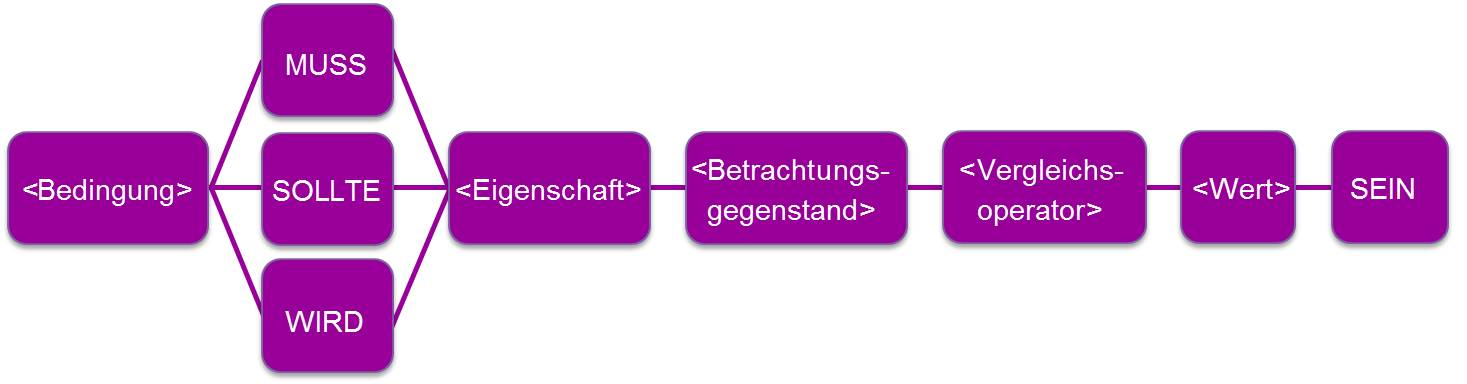
\includegraphics[scale=0.5]{Grafiken/Eigenschafts_Master.jpg}
	\captionof{figure}[Eigenschaftsschablone]{Eigenschaftsschablone\autocite[235]{REuM}}
	
\end{minipage}
\end{center}
%%%%%%%%%%%%%%%%%%%%%%%%

%%%%%%%%%%%%%%%%%%%%%%%%%%%%%%%%%%%%%%%%%%%%%%%%%%%%%%%%%%%%%%%%%%%%%%%%%%%
%%%%%%%%%%%%%%%%%%%%%%%%%%%%%%%%%%%%%%%%%%%%%%%%%%%%%%%%%%%%%%%%%%%%%%%%%%%

\item Diagramme und Modelle

Die Alternative zur Natürlichsprachlichen Dokumentation, ist die Visualisierung mittels Diagrammen und Modellen. Hierfür wurden im Laufe der Jahre eine Vielzahl von unterschiedlichen Standards entwickelt, welche zur Darstellung von unterschiedlichsten Anforderungsarten geeignet sind. Es gibt Tools zum beschreiben von Oberflächen, Datenstrukturen, Prozessen usw.. Die folgende Auflistung von Diagrammen und Modellen stellt eine kleine Auswahl dar und hat nicht den Anspruch auf Vollständigkeit.
\begin{itemize}
\itemsep-8pt
\item Mock-Up
\item UML
\item USE-Case
\item BPMN
\item (e)EPK
\item Klassendiagramme
\item ER Diagramme
\end{itemize}

Hier ist auf die richtige Auswahl des Werkzeugs zu achten. Es muss nicht nur zum beschreiben der Anforderung geeignet sein sondern derjenige der die Anforderung damit umzusetzen versucht muss es auch bedienen können.
So eignen sich Mock-Up's zum beschreiben und dokumentieren von Oberflächen. Mit Hilfe von Use-Case, UML (Unified Modelling Language), (e)EPK (erweiterte Ereignis gesteuerte Prozesskette) , BPMN (Business Process Modelling Notation) lassen sich Funktionale Anforderungen in Form von z.B. Prozessbeschreibungen visualisieren wobei für Daten, Schnittstellen und Berechtigungen neben Klassen- und ER-Diagramm ebenfalls BPMN und UML verwendet werden können.
\end{itemize}
% Das Anforderungsmanagement, dient dazu in einem Projekt das gewünschte Ergebnis schon zu beginn  durch eine

